\documentclass[10pt]{amsart}
\usepackage{amsmath}
\usepackage{amsthm}
\usepackage{tikz}
\usepackage{multicol}
\usetikzlibrary{automata, positioning, arrows}

\newtheorem{itheorem}{Theorem}
\newtheorem{idefinition}{Definition}
\theoremstyle{definition}
\newtheorem*{iexample}{Example}
\theoremstyle{remark}
\newtheorem*{iremark}{remark}

\newenvironment{example}{\begin{center}\begin{minipage}{0.9\textwidth}\begin{iexample}}{\end{iexample}\end{minipage}\end{center}}
\newenvironment{theorem}{\begin{center}\begin{minipage}{0.9\textwidth}\begin{itheorem}}{\end{itheorem}\end{minipage}\end{center}}
\newenvironment{definition}{\begin{center}\begin{minipage}{0.9\textwidth}\begin{idefinition}}{\end{idefinition}\end{minipage}\end{center}}
\newenvironment{remark}{\begin{center}\begin{minipage}{0.9\textwidth}\begin{iremark}}{\end{iremark}\end{minipage}\end{center}}


\title{The Solvability of the Word Problem for Automata Groups}
\author{Arden Rasmussen}
\date{\today}

\newcommand{\Z}{\mathbb{Z}}
\renewcommand{\sp}{\textvisiblespace}

\begin{document}

\maketitle

\section{Introduction}%
\label{sec:Introduction}

The word problem in group theory is the question of if two products of
generators are equivalent to the same element of the group. For example
consider the group $D_4$, then the question becomes; are
$rrsrrsr^{-1}ss^{-2}rrs$, and $rsr^{-1}r^{-1}srrrs^{-1}r^{-1}r^{-1}s$ the
same, and given any two elements in the group expressed as a product of the
groups generators, can we determine if they are equivalent?

For an arbitrary group, this is not necessarily possible to determine this for
all elements. However, for automata groups, it has been proven that it is
always possible. When it is possible, we say that the word problem is solvable
for the group. It has been proven that the word problem is solvable for
automata groups, through the use of the Knuth-Bendix method.

\section{Notation}%
\label{sec:Notation}

Before we can begin into the structure of the proof of the solvability of the
word problem, we first need to define some key concepts that will be used
throughout the reset of the paper.

First, we are only focusing on finitely generated groups, which are the groups
where every element can be written as a combination of a finite number of
elements from a finite set of generators. This means that every group that we
will be considering can be presented by generators and relations. For some
group $G$, the set of generators will be denoted $X$, and the set of relations
will be denoted $R$. First we will denote the set of generators union their
inverse the \textit{alphabet}, and denote it as $\Sigma$, so
\begin{align*}
  \Sigma=X\cup X^{-1}.
\end{align*}
Elements of the alphabet are typically called \textit{letters}.

The second thing to define is the \textit{language}. This is the free monoid of the
alphabet, under the group operation.

\begin{definition}
  The free monoid of a group is the set, whose elements are all finite
  sequences of elements from the group, including the sequence of zero
  elements, commonly denoted by $\varepsilon$.
\end{definition}

Elements of the language, will be called words. Note that we primarily use the
notation of a group operation that is multiplicative, but the language can also
be constructed using an additive operation, for example
\begin{align*}
  \Sigma^*=\left\{\varepsilon, r, s, r+r, r+s, r+r+r,\ldots\right\}.
\end{align*}

\begin{example}
  Consider $D_4$, whose generators are $X=\left\{r,s\right\}$. Then the
  alphabet $\Sigma$ would be 
  \begin{align*}
    \Sigma=X\cup X^{-1}=\left\{r,s,r^{-1},s^{-1}\right\}.
  \end{align*}
  Finally the language would be the free monoid of the alphabet
  \begin{align*}
    \Sigma^*=\left\{\varepsilon, r, s, rr,rs,rrr,rrs,\ldots\right\}.
  \end{align*}
  A word in this language could be $rrrsr^{-1}ss^{-1}$.
\end{example}

Since every element of a group can be defined as a product of the groups
generators, then we will call some word $w\in\Sigma^*$, a representation of an
element $a\in G$, if $w=a$.

The last notation that we must define is \textit{shortlex ordering}. This is a
method to apply ordering to the elements of a language.

\begin{definition}
  Words are sorted by length with the shortest words first, and words of the
  same length are sorted into lexicographical order (alphabetical).
\end{definition}

Generally this is just alphabetical ordering, similar to how a dictionary will
order the words in it.

\begin{example}
  For our example of $D_4$, the shortlex ordering is given by
  \begin{align*}
    \varepsilon < r < s < rr < rs < rrr < rrs < \cdots
  \end{align*}
\end{example}

\section{The Word Problem}%
\label{sec:The Word Problem}

The word problem generally stated is to determine if two words are equivalent.
More commonly discussed is the solvability of the word problem, as actually
solving it usually results in large computations, it is beneficial to determine
if the word problem is solvable before actually solving it. More commonly
discussed is the solvability of the word problem, as actually solving it.

\begin{definition}
  The word problem for a finitely generated group $G$ is solvable if for two
  representations of elements in that group $w,u\in\Sigma^*$, then it is
  possible to determine if $w=u$.
\end{definition}

At first this may seem trivial, to state whether two elements are the same, or
not. However, it has been proven that the word problem is not universally
solvable. That is to say, given some arbitrary group, it may not be possible to
say if two representations are the same element or not. However, in specific
groups it has been shown to be solvable.

Returning to the previous example of $rrsrrsr^{-1}ss^{-2}rrs$, and
$rsr^{-1}r^{-1}srrrs^{-1}r^{-1}r^{-1}s$ in $D_4$. These elements appear very
different, however upon evaluation, they are actually equivalent, and both of
these represent the identity element in $D_4$.

\section{Solvability of the Word Problem for $Z_3$}%
\label{sec:Solvability of the Word Problem for $Z_3$}

Proving the word problem is solvable for the Cyclic group of order 3 is
relatively simple, and so we will use it to explain the concept more generally.

\begin{align}
  Z_3=\langle x \vert x^3=1 \rangle
\end{align}
In this group, our alphabet consists of $\Sigma=\left\{x,x^{-1}\right\}$, and
so $\Sigma^*$ is the set of all words combining any number of the letters $x$
and $x^{-1}$. The first step is to write out the relations that we know. The
relations in $Z_3$ provide us with a list of strings that can be inserted or
canceled out whenever they appear in the string, without altering the
represented element of the group. In this case, the relations are listed below.
\begin{multicols}{2}
  \begin{enumerate}
    \item $xxx= e$\label{enum:z3:1}
    \item $xx^{-1}= e$\label{enum:z3:2}
    \item $x^{-1}x= e$\label{enum:z3:3}
    \item $x^{-1}x^{-1}x^{-1}= e$\label{enum:z3:4}
    \item $x^{-1}= xx$\label{enum:z3:5}
    \item $x^{-1}x^{-1}= x$\label{enum:z3:6}
  \end{enumerate}
\end{multicols}
The first relation is derived directly from the definition of $Z_3$. The second
and third come from the definition of an inverse of the element $x$. Relation
\ref{enum:z3:4} is a result that since the cube of $x$ is the identity, then so
is the cube of the inverse of $x$. Relation \ref{enum:z3:5} and \ref{enum:z3:6}
come as a result of multiplying by $e$, and from relation \ref{enum:z3:1},
expanding this out to be of the form $xxxx^{-1}$ and $xxxx^{-1}x^{-1}$
respectively, then by relation \ref{enum:z3:2} we cancel elements are are left
with $xx$ and $x$ respectively.

With these relations we can reduce any string to either be the empty string
$e$, $x$, or $xx$. And thus the word problem is solvable for $Z_3$. 

\begin{example}
  Let us test this by considering $w=xxx^{-1}xx^{-1}x^{-1}xxxx$.
  \begin{align*}
    w&=xxx^{-1}xx^{-1}x^{-1}xxxx\\
    (\ref{enum:z3:2})&\rightarrow xxxx^{-1}x^{-1}xxxx\\
    (\ref{enum:z3:1})&\rightarrow x^{-1}x^{-1}xxxx\\
    (\ref{enum:z3:3})&\rightarrow x^{-1}xxx\\
    (\ref{enum:z3:3})&\rightarrow xx\\
  \end{align*}
  Thus we see that $w=xx=x^2$, and our relations successfully reduced the word
  to the element of the group which it represents. This process can be done for
  any word in $\Sigma^*$.

  So we can consider two arbitrary elements $w,u\in\Sigma^*$. By the relations,
  and the process outlined above, we can reduce $w,u$ to be one of $e,x,xx$,
  let us call the results of this reduction $w',u'$ respectively. Then if
  $w'=u'$, then we can conclude
  \begin{align*}
    w=w'=u'=u.
  \end{align*}
\end{example}


\section{Knuth-Bendix Method}%
\label{sec:Knuth-Bendix Method}

The Knuth-Bendix method is an algorithm that is used to construct the relations
that we will use to solve the word problem. The general concept of the
algorithm is that given a set of equations between terms, it will attempt to
construct a set of relations which encapsulate all the information of the
provided relations, but in a more simplified format. The new writing system is
constructed such that only $e=e$, and no other presentation of elements in the
group $G$ is equivalent to $e$. Thus if it the Knuth-Bendix algorithm succeeds,
then the word problem has been solved, for that group.

Note, even if the Knuth-Bendix algorithm does not succeed, this does not mean
that the word problem is unsolvable for the group. There are other methods that
can be used to solve the algorithm, which may work.

In our example of $Z_3$, we took our original writing system that consisted of
some number of $x$ and $x^{-1}$ in any order, and rewrote it into one of
$\left\{e, x, x^2\right\}$. However, in our example we constructed the
relations manually. In more complex groups constructing all of the relations
manually would not be feasible, and thus we would use the Knuth-Bendix method
to construct the relations, that would then in turn be used to rewrite the
strings into the new writing systems. Once the strings have been rewritten, it
is trivial to check if it is the identity, and thus the word problem has been
solved.

A key component that the Knuth-Bendix method resolves is the lack of
confluence for a set of relations. The confluence of a set of relations,
describes the fact that there are multiple ways to achieve the same result.
Particularly once can apply the relations in different orders and still achieve
the same result. The Knuth-Bendix method develops a set of relations such that
confluence is always preserved. This is crucial to make the problem more
computationally friendly, and thus applicable to automata.

Consider the finitely presented monoid $M=\langle \Sigma\vert R\rangle$, where
$\Sigma$ is the set of generators, and $R$ is the set of relations. First we
will consider the set of all possible words denoted $\Sigma^*$. Now we apply the
concept of shortlex ordering to $\Sigma^*$ to define an ordering on $\Sigma^*$,
which we will denote using $<$.

The first step in the algorithm is to construct our initial set of relations.
To do this consider $P_i=Q_i\in R$, without loss of generality assume
$Q_i<P_i$, then we define the relation $P_i\rightarrow Q_i$, for all $i$.

The next step is to progressively construct new relations to remove the
dependence on relations that do not preserve confluence. Consider some
$P_i,P_j$ with $i\neq j$, that have some overlap. There are two cases for $P_i$
and $P_j$ to overlap.
\begin{enumerate}
  \item Either the prefix of $P_i$ is equal to the suffix of $P_j$ or the
    reverse is true. We can write $P_i=BC$ and $P_j=AB$ in the first case and
    $P_i=AB$ and $P_j=BC$ in the second.
  \item Either $P_i$ is contained entirely within $P_j$ or $P_j$ is contained
    within $P_i$, In this case we write $P_i=B$, and $P_j=ABC$ in the first
    case, and $P_i=ABC$ and $P_j=B$ in the second.
\end{enumerate}
Now we reduce the word given by $ABC$ by using $P_i$ and call this result
$r_i$. We do the same for $P_j$ to get $r_j$. If $r_i\neq r_j$, then we have a
new relation which we will define by
\begin{align*}
  \max\left\{r_i,r_j\right\}\rightarrow\min\left\{r_i,r_j\right\}
\end{align*}
After adding this new rule, remove any relations that have a reducible left
side. This process is repeated until no relations have reducible left sides.

If the Knuth-Bendix method succeeds, then we can conclude that the word problem
is solvable for that group. As with the knuth bendix method, we are able to
rewrite any words in the language, into their most reduced form by the
rewriting system. Then once they are in that form, comparison of these
elements are trivial, as the preservation of confluence guarantees that each
element that cannot be reduced any further must be distinct from one another.
So with this rewriting system constructed, we are able to conclude that the
word problem is solvable for this group. However, to solve it will take a bit
more work.

\subsection{Example}%
\label{sub:example}

Let us consider a very simplistic example and use the Knuth-Bendix algorithm to
rewritten the relations. We will consider the monoid given by
\begin{align*}
  \langle x,y\vert x^3=y^3={(xy)}^3=1\rangle.
\end{align*}
To begin with there are three reductions that have been defined
\begin{align*}
  x^3&\rightarrow1\quad&(1)\\
  y^3&\rightarrow1\quad&(2)\\
  xyxyxy&\rightarrow1\quad&(3)
\end{align*}

Considering $P_1$ and $P_3$ we see that there is some overlap, so we will
consider the word $x^3yxyxy$, and attempt to reduce that.
\begin{align*}
  x^3yxyxy\xrightarrow{(1)}yxyxy\quad\quad
  x^3yxyxy\xrightarrow{(3)}x^2\\
\end{align*}
since we cannot reduce $yxyxy$ or $x^2$ further with our given relations, we
must construct a new relation. By shortlex ordering $x^2<yxyxy$, so this will
be given by
\begin{align*}
  yxyxy&\rightarrow x^2\quad&(4)
\end{align*}

Now we repeat the process with $P_2$ and $P_3$ and consider the word
$xyxyxy^3$.
\begin{align*}
  xyxyxy^3\xrightarrow{(1)}xyxyx\quad\quad
  xyxyxy^3\xrightarrow{(3)}y^2\\
\end{align*}
Thus resulting in the relation
\begin{align*}
  xyxyx&\rightarrow y^2\quad&(5)
\end{align*}

Now there are no other existing overlaps. We first notice that $xyxyxy$ can be
reduced, so we eliminate that relation. Now the set of relations is given by
\begin{align*}
  x^3&\rightarrow1\quad&(1)\\
  y^3&\rightarrow1\quad&(2)\\
  yxyxy&\rightarrow x^2\quad&(4)\\
  xyxyx&\rightarrow y^2\quad&(5)
\end{align*}
Now we repeat the entire process again.

Considering $P_1$ and $P_5$, we will consider the word $x^3yxyx$, and $xyxyx^3$.
\begin{align*}
  x^3yxyx\xrightarrow{(1)}yxyx&\quad\quad
  x^3yxyx\xrightarrow{(5)}x^2y^2\\
  xyxyx^3\xrightarrow{(1)}xyxy&\quad\quad
  xyxyx^3\xrightarrow{(5)}y^2x^2\\
  yxyx&\rightarrow x^2y^2\quad&(6)\\
  y^2x^2&\rightarrow xyxy\quad&(7)
\end{align*}
Considering $P_2$ and $P_4$, we will consider the word $y^3xyxy$ and $yxyxy^3$.
\begin{align*}
  y^3xyxy\xrightarrow{(1)}xyxy&\quad\quad
  y^3xyxy\xrightarrow{(4)}y^2x^2\\
  yxyxy^3\xrightarrow{(1)}yxyx&\quad\quad
  yxyxy^3\xrightarrow{(4)}x^2y^2\\
  yxyx&\rightarrow x^2y^2\quad&(6)\\
  y^2x^2&\rightarrow xyxy\quad&(7)
\end{align*}

Once again we notice that the left hand side of $(4)$ and $(5)$ can be reduced
using these two new relations, so those two relations are removed. Meaning our
set of relations is now
\begin{align*}
  x^3&\rightarrow1\quad&(1)\\
  y^3&\rightarrow1\quad&(2)\\
  yxyx&\rightarrow x^2y^2\quad&(6)\\
  y^2x^2&\rightarrow xyxy\quad&(7)
\end{align*}

Repeating the process for this new set of relations, we will be considering the
words $yxyx^3$, $y^3xyx$, $y^2x^3$, and $y^3x^2$.
\begin{align*}
  yxyx^3\xrightarrow{(1)}yxy&\quad\quad
  yxyx^3\xrightarrow{(6)}x^2y^2x^2\\
  x^2y^2x^2&\rightarrow yxy\quad&(8)\\
  y^3xyx\xrightarrow{(2)}xyx&\quad\quad
  y^3xyx\xrightarrow{(6)}y^2x^2y^2\\
  y^2x^2y^2&\rightarrow xyx\quad&(9)\\
  y^2x^3\xrightarrow{(1)}y^2&\quad\quad
  y^2x^3\xrightarrow{(7)} xyxyx\\
  yxyxyx&\rightarrow x^2\quad&(10)\\
  y^3x^2\xrightarrow{(2)}x^2&\quad\quad
  y^3x^2\xrightarrow{(7)}yxyxy\\
  yxyxy&\rightarrow x^2\quad&(11)\\
\end{align*}
Now we remove all relations whos left side is reducible, this would be $(8)$,
$(9)$, $(10)$, $(11)$, $(8)$ and $(9)$ are reducible by $(7)$, and $(10)$, and
$(11)$ are reducible by $(6)$. Thus we can conclude that the final set of
relations are
\begin{align*}
  x^3&\rightarrow1\quad&(1)\\
  y^3&\rightarrow1\quad&(2)\\
  yxyx&\rightarrow x^2y^2\quad&(6)\\
  y^2x^2&\rightarrow xyxy\quad&(7)
\end{align*}

\section{Finite State Automata}%
\label{sec:Finite State Automata}

To actually solve the word problem for a given group, we will use a finite
state automaton.

\begin{definition}
  A Finite State Automaton is defined as the quintuple $\left(\Sigma, S, s_0,
    \delta, F\right)$. Where $\Sigma$ is the alphabet of symbols, $S$ is a
  non-empty finite set of states, $s_0$ is the initial state such that $s_0\in
  S$, $\delta$ is the state-transition function $\delta:S\times\Sigma\rightarrow
  S$, and $F$ is the finite set of states $F\subseteq S$.
\end{definition}

The set $F$ is the set of states that we want the automaton to
recognize, for example if $F=\left\{1\right\}$, will mean that the automaton
recognizes representations of the identity element. However, the $F$ term can
also be omited, which we will be doing, as we do not yet want our automaton to
tell us if it accepts or rejects an input, but rather manipulate its input.

Since the automaton that we will be working with are deterministic, then there
is exactly one output for every input. So we can consider the automaton $A$ as
a mapping $A:\Sigma^*\rightarrow S$.

\begin{example}
\begin{figure}[htpb]
  \begin{center}
    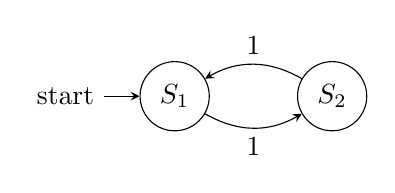
\begin{tikzpicture}[scale=1, transform shape,->,>=stealth]
      \node[state, initial] at (-1,0) (s1) {$S_1$};
      \node[state] at (1,0) (s2) {$S_2$};
      \draw (s1) edge[bend right, below] node{$1$} (s2);
      \draw (s2) edge[bend right, above] node{$1$} (s1);
    \end{tikzpicture}
  \end{center}
  \caption{Very simple Finite state automata}%
  \label{fig:auto_ex}
\end{figure}

Consider the Finite State Automaton presented in figure \ref{fig:auto_ex}. For
this automaton $\Sigma=\left\{0, 1\right\}$, $S=\left\{S_1,S_2\right\}$,
$s_0=S_1$, and
\begin{align*}
  \delta(s, l) = \begin{cases}
    S_1 & \text{if }s=S_2\text{ and }l=1\\
    S_2 & \text{if }s=S_1\text{ and }l=1
  \end{cases}.
\end{align*}

Note that the explicit format for $\delta$ can be relatively complex, so it is
common to express the transition function as a table. Thus the transition table
for this automaton is given in Table \ref{tab:auto_ex}.

\begin{table}[htpb]
  \centering
  \caption{Transition table for Figure\ref{fig:auto_ex}.}\label{tab:auto_ex}
  \begin{tabular}{c||c}
    $\delta$ & 1\\
    \hline\hline
    $S_1$ & $S_2$\\
    \hline
    $S_2$ & $S_1$\\
  \end{tabular}
\end{table}

We can use this table to determine the output of the finite state automaton.
Let us consider the example where $w\in\Sigma^*$, with $w=1111$. Running the
automaton with this input of $w$ we see that each stage is described below
\begin{multicols}{2}
  \begin{enumerate}
    \item $s=S_1$, $w=1111$.
    \item $s=S_2$, $w=111$.
    \item $s=S_1$, $w=11$.
    \item $s=S_2$, $w=1$.
    \item $s=S_1$, $w=\epsilon$.
  \end{enumerate}
\end{multicols}

Thus after the automaton has been run on the input of $w$ the output of the
automaton is $S_1$. We can see that this automaton is actually representative
of $\Z/2\Z$, when we replace $S_1$ with $0$, ad $S_2$ with $1$.
\end{example}

To construct an automaton from a group, let us consider the group $D_4$. $D_4$
is presented by the generators and relations $\langle a,b | a^4=1, b^2=1,
(ab)^2=1\rangle$. We will denote the states, to be the words which cannot be
rewritten any further, by the rewriting system, thus $S=\left\{e,a,a^2,a^3,b,ab,a^2b,a^3b\right\}$. Now we consider
our $X=\left\{a,b\right\}$. Then we find
$\Sigma=\left\{a,a^{-1},b,b^{-1}\right\}$. And finally the transition table for
$D_4$ is given in table \ref{tab:d4};

\begin{table}[htpb]
  \centering
  \caption{Transition table for $D_4$}
  \label{tab:d4}
  \begin{tabular}{c||c|c|c|c}
    $\delta_{D_4}$ & $a$ & $a^{-1}$ & $b$ & $b^{-1}$\\
    \hline\hline
    $e$ & $a$ & $a^3$ & $b$ & $b$\\
    $a$ & $a^2$ & $e$ & $a^3b$ & $a^3b$\\
    $a^2$ & $a^3$ & $a$ & $a^2b$ & $a^2b$\\
    $a^3$ & $e$ & $a^2$ & $ab$ & $ab$\\
    $b$ & $ab$ & $a^3b$ & $e$ & $e$\\
    $ab$ & $a^2b$ & $b$ & $a^3$ & $a^3$\\
    $a^2b$ & $a^3b$ & $ab$ & $a^2b$ & $a^2b$\\
    $a^3b$ & $b$ & $a^2b$ & $a$ & $a$\\
  \end{tabular}
\end{table}

Using this table, and the states, we can construct the diagram representing the
automaton for $D_4$.

\begin{figure}[htpb]
  \begin{center}
    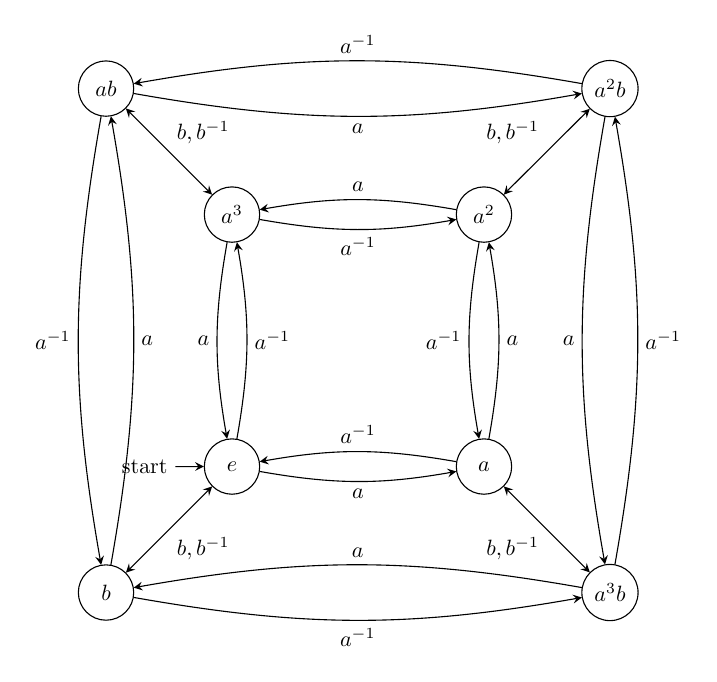
\begin{tikzpicture}[scale=0.8, transform shape,->,>=stealth]
      \node[state, initial] at (-2,-2) (e) {$e$};
      \node[state] at (2,-2) (a) {$a$};
      \node[state] at (2,2) (a2) {$a^2$};
      \node[state] at (-2,2) (a3) {$a^3$};

      \node[state] at (-4,-4) (b) {$b$};
      \node[state] at (-4,4) (ab) {$ab$};
      \node[state] at (4,4) (a2b) {$a^2b$};
      \node[state] at (4,-4) (a3b) {$a^3b$};

      \draw (e) edge[bend right=10, below] node{$a$} (a);
      \draw (a) edge[bend right=10, right] node{$a$} (a2);
      \draw (a2) edge[bend right=10, above] node{$a$} (a3);
      \draw (a3) edge[bend right=10, left] node{$a$} (e);
      \draw (e) edge[bend right=10, right] node{$a^{-1}$} (a3);
      \draw (a3) edge[bend right=10, below] node{$a^{-1}$} (a2);
      \draw (a2) edge[bend right=10, left] node{$a^{-1}$} (a);
      \draw (a) edge[bend right=10, above] node{$a^{-1}$} (e);

      \draw (e) edge[below right,<->] node{$b,b^{-1}$} (b);
      \draw (a) edge[below left,<->] node{$b,b^{-1}$} (a3b);
      \draw (a2) edge[above left,<->] node{$b,b^{-1}$} (a2b);
      \draw (a3) edge[above right,<->] node{$b,b^{-1}$} (ab);

      \draw (b) edge[bend right=10, right] node{$a$} (ab);
      \draw (ab) edge[bend right=10, below] node{$a$} (a2b);
      \draw (a2b) edge[bend right=10, left] node{$a$} (a3b);
      \draw (a3b) edge[bend right=10, above] node{$a$} (b);
      \draw (ab) edge[bend right=10, left] node{$a^{-1}$} (b);
      \draw (a2b) edge[bend right=10, above] node{$a^{-1}$} (ab);
      \draw (a3b) edge[bend right=10, right] node{$a^{-1}$} (a2b);
      \draw (b) edge[bend right=10, below] node{$a^{-1}$} (a3b);
    \end{tikzpicture}
  \end{center}
  \caption{Finite state automaton for $D_4$}%
  \label{fig:d4}
\end{figure}

With this automaton representation of $D_4$ we can consider any sequence of
generators $w\in\Sigma^*$, and determine the reduced representation of this
element, we just need to apply the automaton as we did in the prior example.
Since we apply the automaton to words in the laguange, lets consider the word
$w=aabaaba^{-1}bb^{-1}aab$. Then to apply the automaton, we first start with
$A_e(aabaaba^{-1}bb^{-1}aab)$, where the $A_e$ denotes the automaton in state
$e$. Then by considering the first letter of the word, and the current state of
the automaton, we use the transition function to determine what state the
automaton should be at next. In this case $\delta(e,a)=a$, so the next state
will be $a$. Once a letter of the word has been read, it can be removed, so
after this first step is done, we now write the expression
$A_a(abaaba^{-1}bb^{-1}aab)$. 

\begin{align*}
  A_1(aabaaba^{-1}bb^{-1}aab)&\xrightarrow{\delta(1,a)=a}A_a(abaaba^{-1}bb^{-1}aab)\\
  \xrightarrow{\delta(a,a)=a^2}A_{a^2}(baaba^{-1}bb^{-1}aab)
  &\xrightarrow{\delta(a^2,b)=a^2b}A_{a^2b}(aaba^{-1}bb^{-1}aab)\\
  \xrightarrow{\delta(a^2b,a)=a^3b}A_{a^3b}(aba^{-1}bb^{-1}aab)
  &\xrightarrow{\delta(a^3b,a)=b}A_{b}(ba^{-1}bb^{-1}aab)\\
  \xrightarrow{\delta(b,b)=e}A_{e}(a^{-1}bb^{-1}aab)
  &\xrightarrow{\delta(e,a^{-1})=a^3}A_{a^3}(bb^{-1}aab)\\
  \xrightarrow{\delta(e,a^{-1})=a^3}A_{a^3}(bb^{-1}aab)
  &\xrightarrow{\delta(a^3,b)=ab}A_{ab}(b^{-1}aab)\\
  \xrightarrow{\delta(ab,b^{-1})=a^3}A_{a^3}(aab)
  &\xrightarrow{\delta(a^3,a)=e}A_{e}(ab)\\
  \xrightarrow{\delta(e,a)=a}A_{a}(b)
  &\xrightarrow{\delta(a,b)=a^3b}A_{a^3b}()\\
\end{align*}

Then when all letters of the word have been read, then the state of the
automaton is the output, and in this case that means that $w=a^3b$, and that
$a^3b$ is the normal form for our sample $w$.

\section{Using the Finite State Automata}%
\label{sec:Using the Finite State Automata}

Now that we have constructed what a finite state automata is, we will develop a
method to construct the automaton from the rewriting system constructed by the
knuth-bendix method. Our alphabet, will be the same alphabet that was used by
the knuth bendix method, then the set of states will be the set of normal forms
for the set, or the set of words which cannot be rewritten any further. The
initial state will remain as the identity.

The transition function for the automaton is somewhat more complected to
construct, but the general premise is to append the letter to the word 
represented by the state, unless there is a rewriting rule that could be used
on this new word. If there is, then we will instead goto the word defined by
applying that rewriting rule to the state.

\subsection{Example}
\label{sub:fsa_example}

Lets consider the group $D_3=\left\langle x,y\vert
  x^3=y^2=(xy)^2=1\right\rangle$. After applying the knuth-bendix method to
this group, we are given the set of rewriting rules:
\begin{align*}
  y^2&\rightarrow1\quad&(2)\\
  xx^{-1}&\rightarrow1\quad&(3)\\
  x^{-1}x&\rightarrow1\quad&(4)\\
  x^2&\rightarrow x^{-1}\quad&(8)\\
  x^{-1}x^{-1}&\rightarrow x\quad&(9)\\
  y^{-1}&\rightarrow y\quad&(10)\\
  yx&\rightarrow x^{-1}y\quad&(15)\\
  yx^{-1}&\rightarrow xy\quad&(16)
\end{align*}

Now to construct the transitions function, we simply go through every state,
and append each possible letter of the alphabet to the word for that state, if
there are rules to rewrite the resulting word, then do so. Using this process
we get the automaton shown in figure~\ref{fig:d3}.

\begin{figure}[htpb]
  \begin{center}
    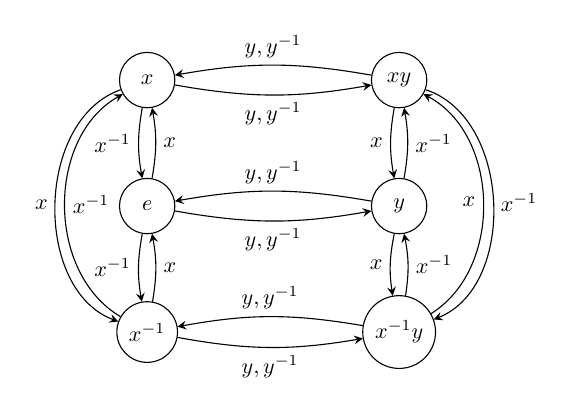
\begin{tikzpicture}[scale=0.8, transform shape,->,>=stealth]
      \node[state] at (-2,0) (e) {$e$};
      \node[state] at (-2,2) (x) {$x$};
      \node[state] at (-2,-2) (xi) {$x^{-1}$};
      \node[state] at (2,0) (y) {$y$};
      \node[state] at (2,2) (xy) {$xy$};
      \node[state] at (2,-2) (xiy) {$x^{-1}y$};

      \draw (e) edge[bend right=10, right] node{$x$} (x);
      \draw (e) edge[bend right=10, left] node{$x^{-1}$} (xi);
      \draw (e) edge[bend right=10, below] node{$y,y^{-1}$} (y);

      \draw (x) edge[bend right=70, left] node{$x$} (xi);
      \draw (x) edge[bend right=10, left] node{$x^{-1}$} (e);
      \draw (x) edge[bend right=10, below] node{$y,y^{-1}$} (xy);

      \draw (xi) edge[bend right=10, right] node{$x$} (e);
      \draw (xi) edge[bend left=60, right] node{$x^{-1}$} (x);
      \draw (xi) edge[bend right=10, below] node{$y,y^{-1}$} (xiy);

      \draw (y) edge[bend right=10, above] node{$y,y^{-1}$} (e);
      \draw (y) edge[bend right=10, left] node{$x$} (xiy);
      \draw (y) edge[bend right=10, right] node{$x^{-1}$} (xy);

      \draw (xy) edge[bend right=10, above] node{$y,y^{-1}$} (x);
      \draw (xy) edge[bend right=10, left] node{$x$} (y);
      \draw (xy) edge[bend left=70, right] node{$x^{-1}$} (xiy);

      \draw (xiy) edge[bend right=60, left] node{$x$} (xy);
      \draw (xiy) edge[bend right=10, right] node{$x^{-1}$} (y);
      \draw (xiy) edge[bend right=10, above] node{$y,y^{-1}$} (xi);
    \end{tikzpicture}
  \end{center}
  \caption{Finite state automaton for $D_3$, generated by the Knuth-Bendix
    method}\label{fig:d3}
\end{figure}

Once this automaton has been constructed it is now possible to consider the
automaton as a function that maps the word to its normal form, or its most
reduced form according to the rewriting system. Then these normal forms can
compared for equality. Thus we have solved the word problem for automatic
groups.

\nocite{*}
\bibliographystyle{plain}
\bibliography{ref}

\end{document}
